% Motivation model diagram Heckhausen and Rheinberg
% Author: Stefan Kottwitz
\documentclass[tikz,border=10pt]{standalone}
\usepackage[normalem]{ulem}
\tikzset{
  centered/.style = { align=center, anchor=center },
     empty/.style = { font=\sffamily\Large, centered, text width=2cm },
       box/.style = { font=\sffamily, fill=green, centered },
    result/.style = { font=\sffamily\scriptsize, fill=black!20, centered},
     arrow/.style = { very thick, color=red, ->, >=Triangle},
}
\newcommand*{\nothing}{Do nothing}

\begin{document}
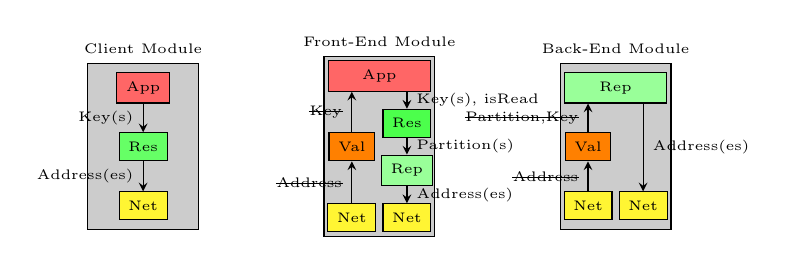
\begin{tikzpicture}
	[layer/.style={rectangle,draw}];
	
	\node (client) at (-3,0) [layer,label={\tiny Client Module},minimum height=60pt,minimum width=40pt,fill=black!20] {};
	\node (front) at (0,0) [layer,label={\tiny Front-End Module},minimum height=65pt,minimum width=40pt,fill=black!20] {};
	\node (back) at (3,0) [layer,label={\tiny Back-End Module},minimum height=60pt,minimum width=40pt,fill=black!20] {};
	\node (app1) at (-3,0.75) [layer,fill=red!60] {\tiny App};
	\node (resolution1) at (-3,0) [layer,fill=green!60] {\tiny Res};
	\node (network1) at (-3,-0.75) [layer,fill=yellow!80] {\tiny Net};
	
	\draw [-stealth] (app1.south) -- (resolution1.north) node[draw=none,fill=none,font=\scriptsize,midway,left] {\tiny Key(s)};
	\draw [-stealth] (resolution1.south) -- (network1.north) node[draw=none,fill=none,font=\scriptsize,midway,left] {\tiny Address(es)};
	
	\node (network21) at (-0.35,-0.9) [layer,fill=yellow!80] {\tiny Net};
	\node (val2) at (-0.35,0) [layer,fill=red!50!yellow] {\tiny Val};
	\node (app2) at (0,0.9) [layer,fill=red!60,minimum width=37pt] {\tiny App};
	\node (resolution2) at (0.35,0.3) [layer,fill=green!70] {\tiny Res};
	\node (replication2) at (0.35,-0.3) [layer,fill=green!40] {\tiny Rep};
	\node (network22) at (0.35,-0.9) [layer,fill=yellow!80] {\tiny Net};
	
	\draw [-stealth] (network21.north) -- (val2.south) node[draw=none,fill=none,font=\scriptsize,midway,left] {\tiny \sout{Address}};
	\draw [-stealth] (val2.north) -- (-0.35,0.7) node[draw=none,fill=none,font=\scriptsize,midway,left] {\tiny \sout{Key}};
	\draw [-stealth] (0.35,0.7) -- (resolution2.north) node[draw=none,fill=none,font=\scriptsize,midway,right] {\tiny Key(s), isRead};
	\draw [-stealth] (resolution2.south) -- (replication2.north) node[draw=none,fill=none,font=\scriptsize,midway,right] {\tiny Partition(s)};
	\draw [-stealth] (replication2.south) -- (network22.north) node[draw=none,fill=none,font=\scriptsize,midway,right] {\tiny Address(es)};

	\node (network31) at (2.65,-0.75) [layer,fill=yellow!80] {\tiny Net};
	\node (val3) at (2.65,0) [layer,fill=red!50!yellow] {\tiny Val};
	\node (replication3) at (3,0.75) [layer,fill=green!40,minimum width=37pt] {\tiny Rep};
	\node (network32) at (3.35,-0.75) [layer,fill=yellow!80] {\tiny Net};
	
	\draw [-stealth] (network31.north) -- (val3.south) node[draw=none,fill=none,font=\scriptsize,midway,left] {\tiny \sout{Address}};
	\draw [-stealth] (val3.north) -- (2.65,0.55) node[draw=none,fill=none,font=\scriptsize,midway,left] {\tiny \sout{Partition,Key}};
	\draw [-stealth] (3.35,0.55) -- (network32.north) node[draw=none,fill=none,font=\scriptsize,midway,right] {\tiny Address(es)};
\end{tikzpicture}
\end{document}
